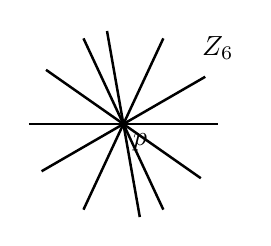
\begin{tikzpicture}[scale=0.4]
% Six lines passing through a common point p at the origin
% Draw the six lines without inline labels
\foreach \theta in {115,-80,65,-35,30,0} {
    \draw[rotate=\theta, line width=0.9pt] (-3,0) -- (3,0);
}
% Common intersection point p
\fill (0,0) circle (2pt) node[below right] {$p$};

% Optional label
\node at (3,2.4) {$Z_6$};
\end{tikzpicture}